\subsection{Bayes Classifier}

\begin{frame}
  \frametitle{Bayes rule for classification}
   
   
Classification problem with $K$ classes: $Y \in \mathcal{Y}=\{1,\ldots,K\}$,

\begin{block}{Probability of class $Y=k$ given $X=x$}  
Bayes rule:
  \begin{align*}
 p{(Y=k|X=x)} &=  \frac{ p(x| Y=k)p{(Y=k)} } { p(x) } =
  \frac{p(x| Y=k)p{(Y=k)} } { \sum_{j=1}^K p(x|Y=j)p{(Y=j)}  },\\  
  & = \structuretext{ \frac{  \pi_k \,  p_k(x) } { \sum_{j=1}^K  \pi_j \,  p_j(x)   } }
 \end{align*}
%\begin{block}{Problem}
 \begin{itemize}
  \item \structuretext{$p_k(x) \equiv p(x| Y=k)$} is the {\em density} for $X$ in class $k$
  \item \structuretext{$\pi_k \equiv p{(Y=k)}$} is the {\em weight}, or {\em prior} probability of class $k$  
 \end{itemize}
\end{block}

\end{frame}


\begin{frame}
  \frametitle{Bayes classifier}
  
  \begin{block}{Definition}
  The Bayes classification rule $f^{\ast}$ is defined as
   \structuretext{ \begin{align*}
    f^{\ast}(x)= \arg \max_{k \in\mathcal{Y}  }p( Y= k | X=x).
   \end{align*} }
   \end{block}
 \begin{block}{Theorem}
 The Bayes classification rule $f^{\ast}$ is optimal in the misclassification rate sense where $\mathcal{E}[f]=p( f(X)  \ne Y)$: 
   \structuretext{\centerline{for any rule $f$, $\mathcal{E}[f]  \ge \mathcal{E}[f^{\ast}]$,}}
 \end{block}
  \begin{block}{Remarks}
   \begin{itemize}
    \item $f^{\ast}(X) \equiv$  {\it maximum a posteriori} (MAP) estimate
    \item In real-word applications,  the distribution of $(X,Y)$ is unknown $\Rightarrow$ no analytical expression  of $f^{\ast}(X)$. 
    But useful reference on academic examples.
   \end{itemize}

 \end{block}
\end{frame}




\begin{frame}{Estimation of $f^{\ast}(X)$}
Two kinds of approaches based on a model:
\begin{enumerate}
 %\item Prototype, or ``black box'' approaches $\leftarrow$ direct learning of the classification rule
 \item \textbf{Discriminative approaches}: direct learning  of $p{(Y|X)}$,\\
   e.g. logistic regression
 \item \textbf{Generative models}: learning of the joint distribution $p(X,Y)$
 \begin{align*}
  p(X,Y) &= \underbrace{p(X|Y)}_{\textrm{likelihood}} \underbrace{\Pr{(Y)}}_{\textrm{prior}},
 \end{align*}
e.g. \structuretext{linear/quadratic discriminant analysis}, Naïve Bayes
\end{enumerate}

\end{frame}



\begin{frame}{Generative models: Estimation problem}
\begin{block}{Assumptions}
 \begin{itemize}
  \item classification problem with $K$ classes: $Y \in \mathcal{Y}=\{1,\ldots,K\}$,
  \item input variables: $X \in \mathbb{R}^p$
 \end{itemize}
\end{block}
 Bayes rule:
  \begin{align*}
 p{(Y=k|X=x)} & = \frac{p(x| Y=k)p{(Y=k)} } { \sum_{j=1}^K p(x|Y=j)p{(Y=j)}  }.
 \end{align*}
%\begin{block}{Problem}
 In practice, the following quantities are unknown:
 \begin{itemize}
  \item densities of each class $p_k(x) \equiv p(x| Y=k)$
  \item weights, or prior probabilities, of  each class  $\pi_k \equiv p{(Y=k)}$
 \end{itemize}
%\end{block}

\begin{block}{Estimation problem}
 These quantities must be learned on a training set:\\
 \begin{center}
  {learning problem \alert{ $\Leftrightarrow$ estimation problem} in a parametric or not way }
 \end{center}

\end{block}

\end{frame}


\subsection{Linear/Quadratic Discriminant Analysis}


\begin{frame}{Quadratic Discriminant Analysis (QDA)}
\begin{block}{Supervised classification assumptions}
 \begin{itemize}
  \item $X \in \mathbb{R}^p$, $Y \in \mathcal{Y}=\{1,\ldots,K\}$,
  \item sized $n$ training set $(X_1,Y_1), \ldots (X_n,Y_n)$
 \end{itemize}
\end{block}

\begin{block}{QDA Assumptions}
The input variables $X$, given a class $Y=k$, are distributed according to a parametric and Gaussian distribution:
\begin{align*}
 X|Y=k \ \sim \ \mathcal{N}(\mu_k,\Sigma_k) \  \Leftrightarrow \ p_k(x)= \frac{1}{(2 \pi)^{p/2} |\Sigma_k|^{1/2}}e^{-\frac{1}{2}
 (x-\mu_k)^T \Sigma_k^{-1} (x-\mu_k)}
\end{align*}
\end{block}
The Gaussian parameters are, for each class $k=1,\ldots,K$
\begin{itemize}
 \item mean vectors $\mu_k \in \mathbb{R}^p$,
 \item covariance matrices $\Sigma_k \in \mathbb{R}^{p \times p}$,
 \item[\doigt] set of parameters $\theta_k \equiv \{\mu_k, \Sigma_k\}$, plus the weights $\pi_k$, for $k=1,\ldots,K$.
\end{itemize}

\end{frame}



\begin{frame}
  \frametitle{Example}
\begin{block}{Mixture of $K=3$ Gaussians}
\begin{itemize}
   \item $Y \in \{\textcolor{red}{1},\textcolor{green}{2},\textcolor{blue}{3}\}$
   \item $X \in \mathbb{R}^2$
\end{itemize}
\end{block}

\only<1>{
\begin{center}
  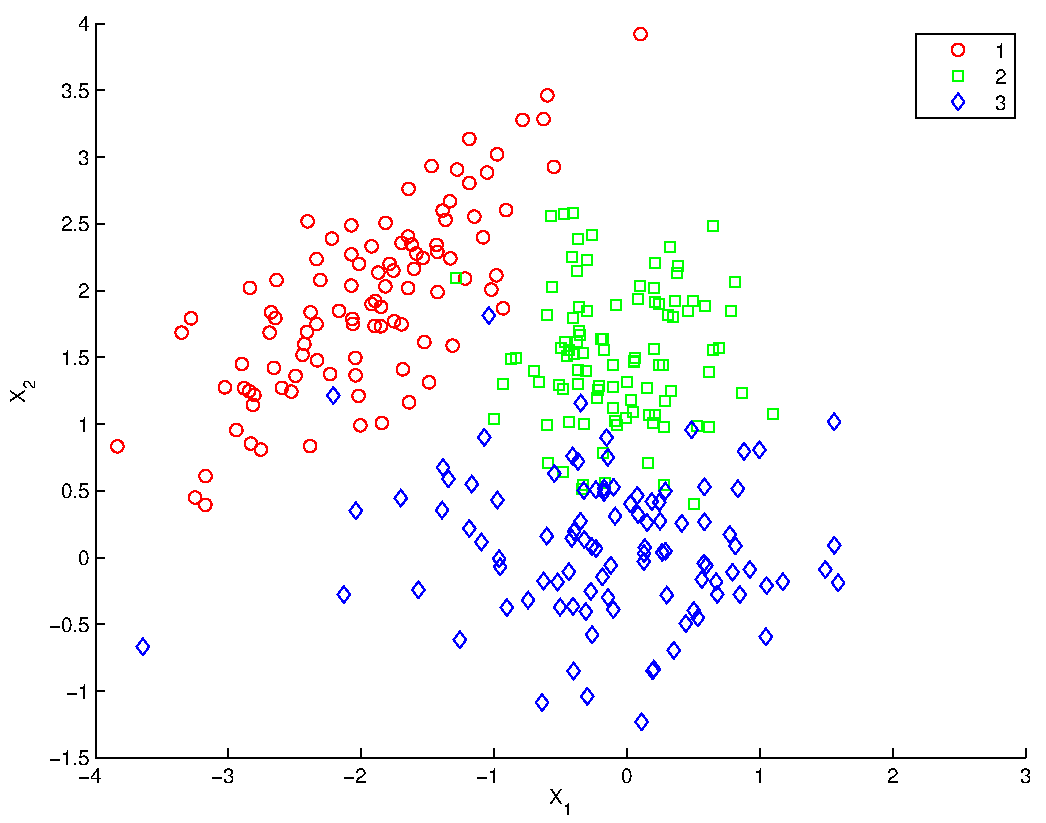
\includegraphics[width=.5\textwidth]{discr_analysis_ex.pdf}
\end{center}}


\only<2>{
\begin{center}
  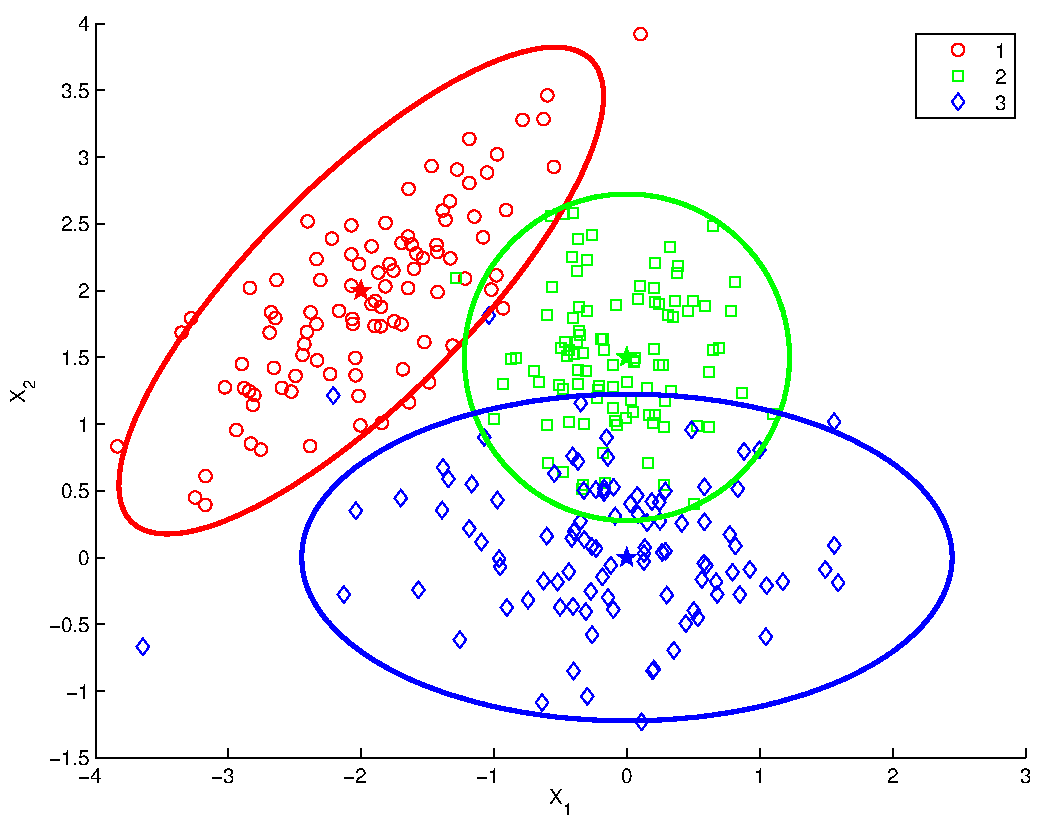
\includegraphics[width=.5\textwidth]{discr_analysis_CI.pdf}
\end{center}}

\end{frame}




\begin{frame}{QDA parameter estimation}

\begin{block}{Notations}
   \begin{itemize}
      \item $n_k= \#\{ y_i=k \}$ is the number of training samples in class $k$,
      \item $\sum_{y_i=k}$ is the sum over all the indices $i$ of the training samples in class $k$
   \end{itemize}
\end{block}


\begin{block}{(Unbiased) Maximum likelihood estimators (MLE)}
\begin{itemize}
 \item $\widehat{\pi}_k = \dfrac{n_k}{n},  \quad \leftarrow $ sample proportion
 \item $\widehat{\mu}_k = \dfrac{\sum_{y_i=k} x_i}{n_k}, \quad \leftarrow $ sample mean
 \item $\widehat{\Sigma}_k = \frac{1}{\structuretext{n_k-1}} \sum_{y_i=k} \left(x_i-\widehat{\mu}_k \right) \left(x_i-\widehat{\mu}_k \right)^T,
 \quad \leftarrow $ sample covariance
\end{itemize}
Rk:  $\frac{1}{n_k-1}$ is a bias correction factor for the covariance MLE (otherwise $\frac{1}{n_k}$)
\end{block}


\end{frame}


\begin{frame}{Discriminant functions}
For model based approaches, Bayes classifier is defined as
$$f^{\ast}(x)= \arg \max_{k \in\mathcal{Y}  }p( Y= k | X=x)$$
\begin{itemize}
 \item equivalent to consider a set of functions $\delta_k(x)$, for $k \in\mathcal{Y}$, derived from a monotone transformation of
 posterior probability $p{(Y=k |X=x)}$
 \item decision boundary  between classes $k$ and $l$ is then defined as the set $\{x \in \mathcal{X}\ : \ \delta_k(x)= \delta_l(x) \}$
\end{itemize}

\begin{block}{Definition}
 $\delta_k(x)$ are called the \structuretext{discriminant functions} of each class $k$
 \begin{itemize}
  \item[\doigt] $x$ is predicted in the $k_0$ class such that  $k_0= \arg \max_{k \in\mathcal{Y} } \delta_k(x) $
 \end{itemize}
\end{block}

\end{frame}


\begin{frame}{QDA decision rule}

The classification rule becomes
\begin{align*}
 f(x)&= \arg \max_{k \in\mathcal{Y}  }p( Y= k | X=x, \widehat{\theta},\widehat{\pi}),\\
 &= \arg \max_{k \in\mathcal{Y}  }
 \underbrace{ \log p( Y= k | X=x, \widehat{\theta},\widehat{\pi} )}_{\structuretext{\delta_k(x)}},
\end{align*}\vspace{-3mm}

\noindent where \vspace{-2mm}
\begin{align*}
 \delta_k(x)= -\frac{1}{2} \log\left|\widehat{\Sigma}_k\right| - \frac{1}{2}
 (x-\widehat{\mu}_k)^T \widehat{\Sigma}_k^{-1} (x-\widehat{\mu}_k)+ \log \widehat{\pi}_k + \cancel{ \textrm{ Cst} },
\end{align*}
is the \structuretext{discriminant function}

\begin{block}{Remarks}
   \begin{enumerate}
      \item different rule than the Bayes classifier as $\theta$  replaced by $\widehat{\theta}$
      (and $\pi$ replaced by  $\widehat{\pi}$)
      \item when $ n \gg p$, $\widehat{\theta} \rightarrow \theta$ (and  $\widehat{\pi} \rightarrow \pi$): convergence to the optimal classifier... only if the Gaussian model is correct!
   \end{enumerate}

\end{block}


\end{frame}


\begin{frame}{QDA decision boundary}
The boundary between two classes $k$ and $l$ is described by the equation
\begin{align*}
\delta_k(x)= \delta_l(x)  \Leftrightarrow \structuretext{ C_{k,l} + L_{k,l}^T x + x^T  Q_{k,l}^T x= 0}, \quad \leftarrow \textrm{\structuretext{quadratic} equation}
\end{align*}
where
\begin{itemize}
 \item $\begin{displaystyle}
        C_{k,l}= { -\frac{1}{2} \log \frac{|\widehat{\Sigma}_k|}{ |\widehat{\Sigma}_l|} + \log \frac{\widehat{\pi}_k}{\widehat{\pi}_l}
        - \frac{1}{2} {\widehat{\mu}_k}^T \widehat{\Sigma}_k^{-1} \widehat{\mu}_k + \frac{1}{2}
 {\widehat{\mu}_l}^T \widehat{\Sigma}_l^{-1} \widehat{\mu}_l},
       \end{displaystyle} \quad \leftarrow \textrm{scalar}$
 \item $\begin{displaystyle}
          L_{k,l}= { \widehat{\Sigma}_k^{-1} \widehat{\mu}_k - \widehat{\Sigma}_l^{-1} \widehat{\mu}_l},
        \end{displaystyle}\quad \leftarrow \textrm{vector in } \mathbb{R}^p$
\item $\begin{displaystyle}
          Q_{k,l}= { \frac{1}{2} \left( -\widehat{\Sigma}_k^{-1} + \widehat{\Sigma}_l^{-1} \right)},
        \end{displaystyle}\quad \leftarrow \textrm{matrix in } \mathbb{R}^{p \times p}$
\end{itemize}

\begin{itemize}
 \item[\doigt] \structuretext{Quadratic discriminant analysis}
\end{itemize}


\end{frame}



\begin{frame}
  \frametitle{QDA example}
\begin{block}{Mixture of $K=3$ Gaussians}
\begin{itemize}
   \item Estimation of the parameters $\hat{\mu}_k$, $\hat{\Sigma}_k$ and $\hat{\pi}_k$, for
   $k= \textcolor{red}{1},\textcolor{green}{2},\textcolor{blue}{3}$
\end{itemize}
\end{block}
\vspace*{-5mm}


\begin{center}
  \only<1>{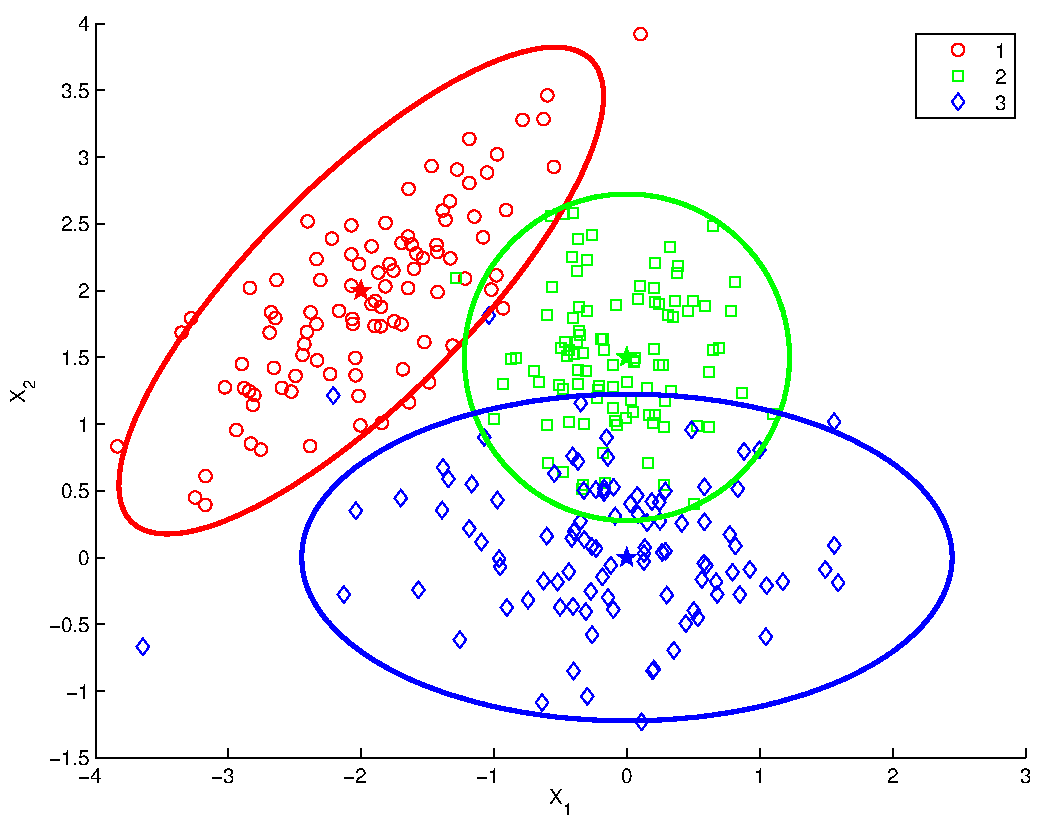
\includegraphics[width=.5\textwidth]{discr_analysis_CI.pdf} \\
  $95\%$ \structuretext{true}  confidence regions}
  \only<2>{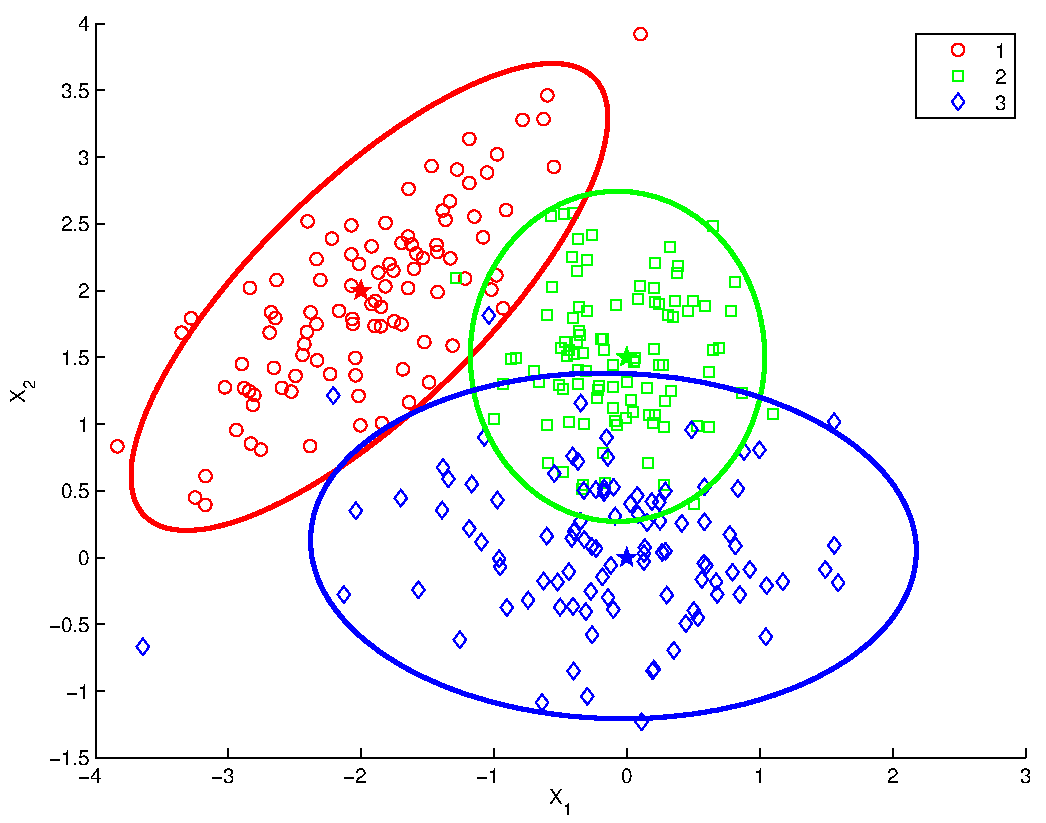
\includegraphics[width=.5\textwidth]{quad_analysis_CI.pdf} \\
  $95\%$ \structuretext{estimated}  confidence regions}
\end{center}

\end{frame}

\begin{frame}
  \frametitle{QDA example (Cont'd)}
\begin{block}{Mixture of $K=3$ Gaussians}
\begin{itemize}
   \item  Classification rule: $\arg \max_{k=\textcolor{red}{1},\textcolor{green}{2},\textcolor{blue}{3}}
\delta_k(x)$
\item Quadratic boundaries $\{ x ; \delta_k(x)=\delta_l(x) \} $
\end{itemize}
\end{block}

\begin{center}
  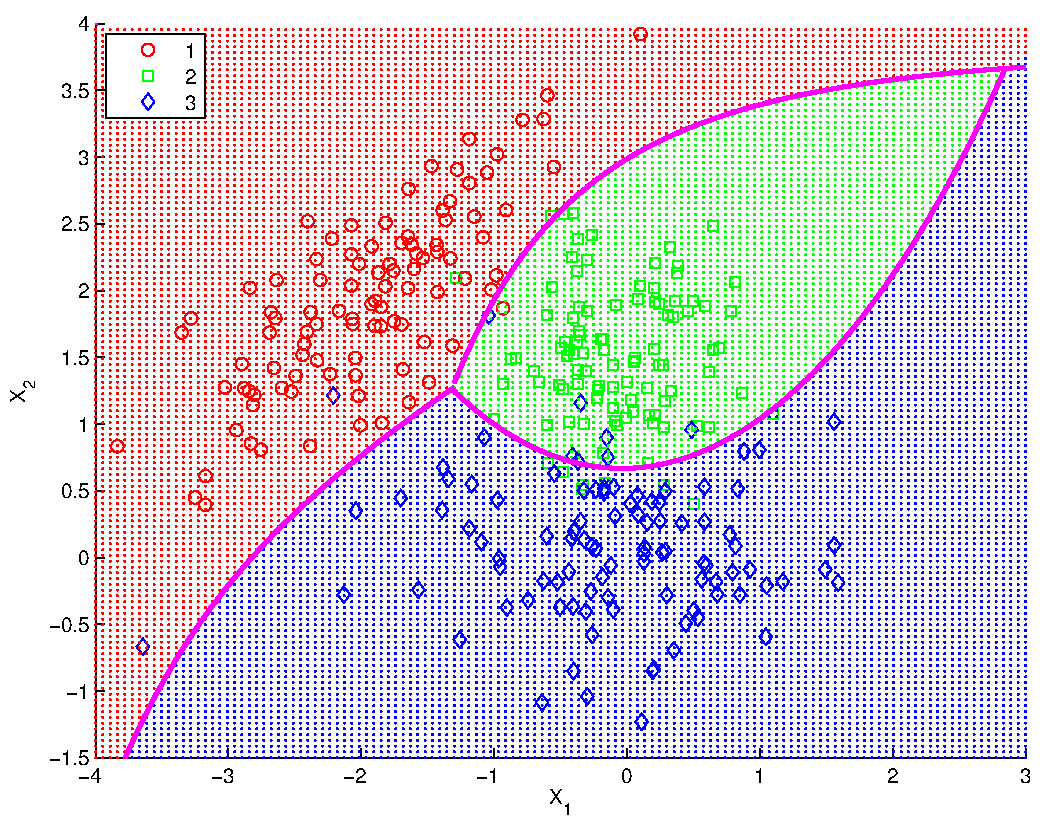
\includegraphics[width=.5\textwidth]{quad_analysis_bounds.pdf} \\
\end{center}

\end{frame}




\begin{frame}{LDA principle}

\begin{block}{LDA Assumptions}
Additional simplifying assumption w.r.t. QDA: all the class covariance matrices are identical (``homoscedasticity''), i.e. \structuretext{$\Sigma_k= \Sigma$}, for $k=1,\ldots,K$
\end{block}\medskip

\begin{block}{(Unbiased) Maximum likelihood estimators (MLE)}
\begin{itemize}
 \item $\widehat{\pi}_k$ and $\widehat{\mu}_k$ are unchanged,
 \item $\widehat{\Sigma} = \frac{1}{\structuretext{n-K}} \sum_{k=1}^K \sum_{y_i=k} \left(x_i-\widehat{\mu}_k \right) \left(x_i-\widehat{\mu}_k \right)^T,
 \quad \leftarrow $ pooled  covariance
\end{itemize}
Rk:  $\frac{1}{n-K}$ is a bias correction factor for the covariance MLE (otherwise $\frac{1}{n}$)
\end{block}\medskip

\begin{block}{LDA discriminant function}
\begin{align*}
 \delta_k(x)&= -\frac{1}{2} \log\left|\widehat{\Sigma}\right| - \frac{1}{2}
 (x-\widehat{\mu}_k)^T \widehat{\Sigma}^{-1} (x-\widehat{\mu}_k)+ \log \widehat{\pi}_k + \cancel{ \textrm{ Cst} },
\end{align*}
\end{block}
\end{frame}



\begin{frame}{LDA decision boundary}
The boundary between two classes $k$ and $l$ reduces to the equation
\begin{align*}
\delta_k(x)= \delta_l(x)  \Leftrightarrow \structuretext{ C_{k,l} + L_{k,l}^T x  = 0 }, \quad \leftarrow \textrm{\structuretext{linear} equation}
\end{align*}
where
\begin{itemize}
 \item $\begin{displaystyle}
        C_{k,l}= {  \log \frac{\widehat{\pi}_k}{\widehat{\pi}_l}
        - \frac{1}{2} {\widehat{\mu}_k}^T \widehat{\Sigma}^{-1} \widehat{\mu}_k + \frac{1}{2}
 {\widehat{\mu}_l}^T \widehat{\Sigma}^{-1} \widehat{\mu}_l},
       \end{displaystyle} \quad \leftarrow \textrm{scalar}$
 \item $\begin{displaystyle}
          L_{k,l}=  \widehat{\Sigma}^{-1} \left( \widehat{\mu}_k -  \widehat{\mu}_l \right),
        \end{displaystyle}\quad \leftarrow \textrm{vector in } \mathbb{R}^p$
\item $\begin{displaystyle}
          Q_{k,l}= \structuretext{0},
        \end{displaystyle}$
\end{itemize}

\begin{itemize}
 \item[\doigt] \structuretext{Linear discriminant analysis}
\end{itemize}


\end{frame}




\begin{frame}
  \frametitle{LDA example}
\begin{block}{Mixture of $K=3$ Gaussians}
\begin{itemize}
   \item Estimation of the parameters  $\hat{\mu}_k$, $\hat{\pi}_k$, for
   $k= \textcolor{red}{1},\textcolor{green}{2},\textcolor{blue}{3}$, and $\hat{\Sigma}$
\end{itemize}
\end{block}
\vspace*{-5mm}

\begin{center}
  \only<1>{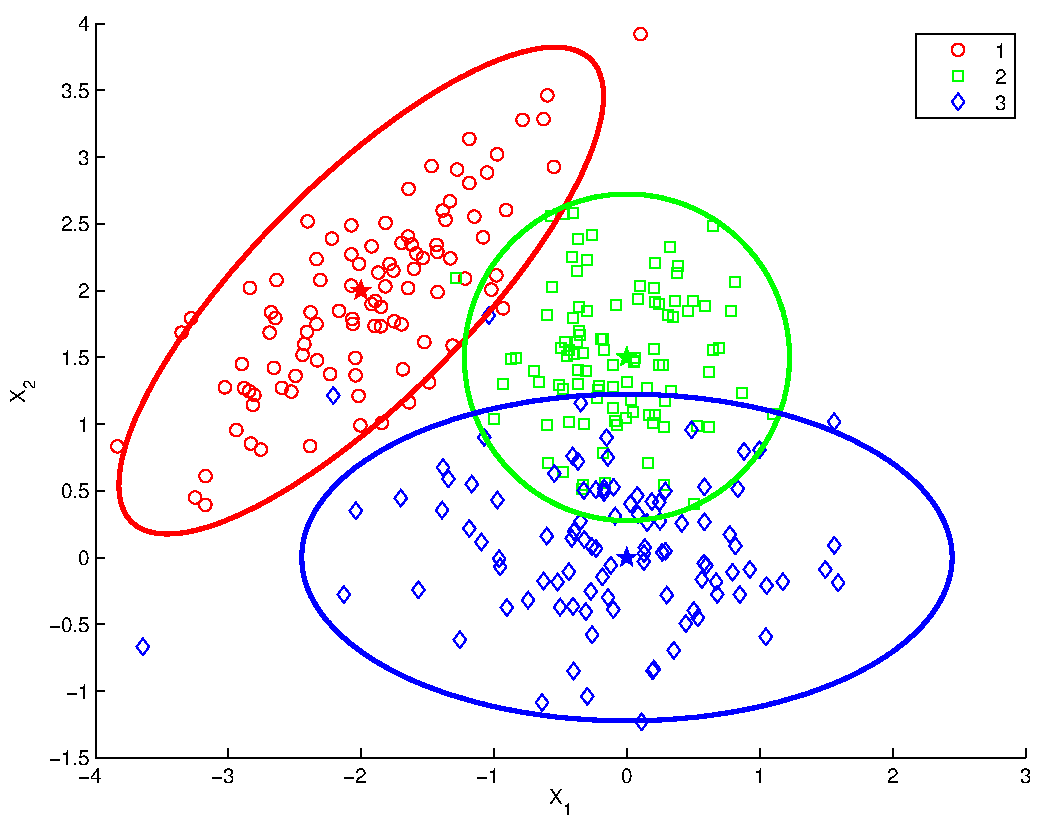
\includegraphics[width=.5\textwidth]{discr_analysis_CI.pdf} \\
  $95\%$ \structuretext{true}  confidence regions}
  \only<2>{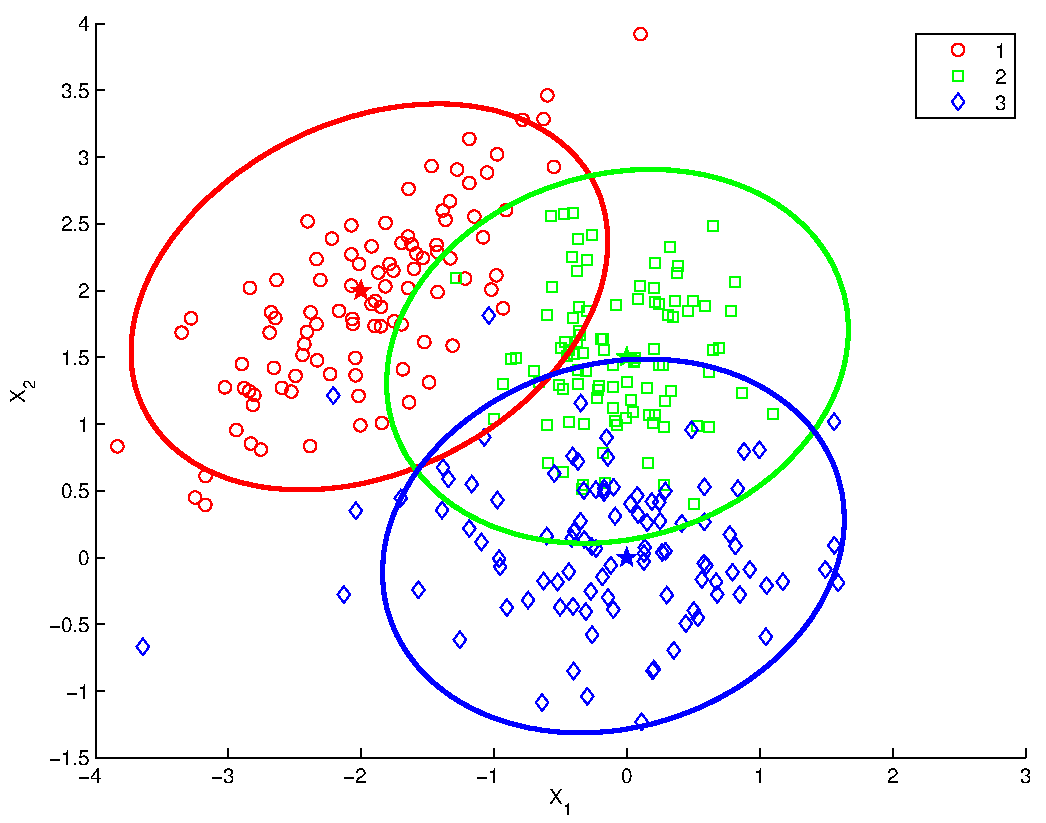
\includegraphics[width=.5\textwidth]{lin_analysis_CI.pdf} \\
  $95\%$ \structuretext{estimated} confidence regions}
\end{center}

\end{frame}


\begin{frame}
  \frametitle{LDA example (Cont'd)}
\begin{block}{Mixture of $K=3$ Gaussians}
\begin{itemize}
   \item  Classification rule:  $\arg \max_{k=\textcolor{red}{1},\textcolor{green}{2},\textcolor{blue}{3}}
\delta_k(x)$
\item linear boundaries $\{ x ; \delta_k(x)=\delta_l(x) \} $
\end{itemize}
\end{block}

\begin{center}
  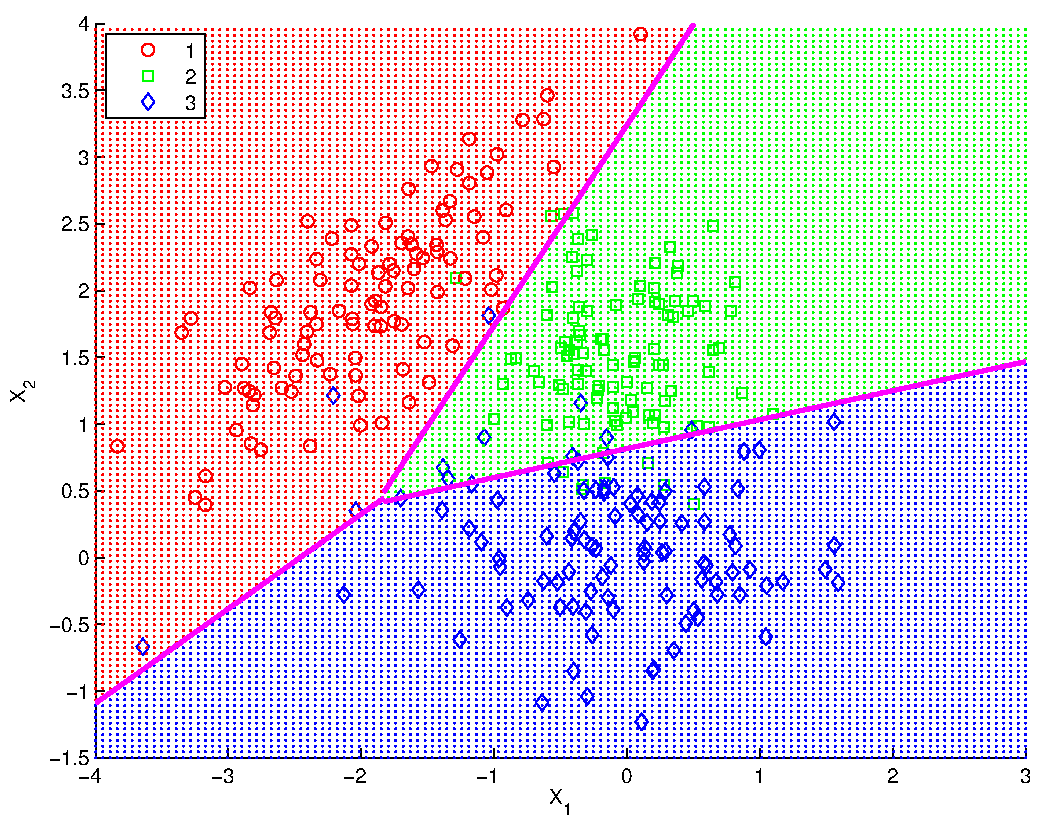
\includegraphics[width=.5\textwidth]{linear_analysis_bounds.pdf} \\
\end{center}

\end{frame}


\begin{frame}{Complexity of discriminant analysis methods}
\begin{block}{Effective number of parameters}
\begin{itemize}
   \item LDA: $(K-1) \times (p+1) = O(Kp)$
   \item QDA: $(K-1) \times \left( \frac{p(p+3)}{2} +1 \right) = O(Kp^2)$
\end{itemize}
\end{block}

\begin{block}{Remarks}
\begin{itemize}
   \item In high dimension, i.e. $p \approx n$  or $p>n$, LDA is more stable than QDA which is more prone to overfitting,
   \item Both methods appear however to be  robust on a large number of real-word datasets
   \item LDA can be viewed in some cases as a least squares regression method
   \item LDA performs a dimension reduction to a subspace of dimension $\le K-1$ generated by
   the vectors $z_k=\Sigma^{-1} \widehat{\mu}_k$  $\leftarrow$ \structuretext{dimension reduction from $p$ to $K-1$}\quad !
\end{itemize}
\end{block}
\end{frame}



%\section{Conclusions}

\begin{frame}{Conclusions on discriminant analysis}
\begin{block}{Generative models}
   \begin{itemize}
      \item learning/estimation of $p(X,Y)= p(X | Y)p{(Y)}$,
      \item derivation of $p{(Y | X)}$ from Bayes rule,
   \end{itemize}
\end{block}
 \begin{block}{Different assumptions on the class densities $p_k(x)=p(X=x|Y=k)$}
      \begin{itemize}
      \item QDA/LDA: Gaussian parametric model
      \item[\doigt] performs well on many real-word datasets
      \item[\doigt] LDA is especially useful when $n$ is small
      \end{itemize}
\end{block}

\begin{block}{Perspectives}
   Model free approaches: direct learning of the prediction rule $f$
\end{block}

\alert{Notebook}

\end{frame}




%%% Local Variables:
%%% mode: latex
%%% TeX-master: "main"
%%% End:
